% Created by tikzDevice version 0.12.6 on 2024-02-25 12:47:53
% !TEX encoding = UTF-8 Unicode
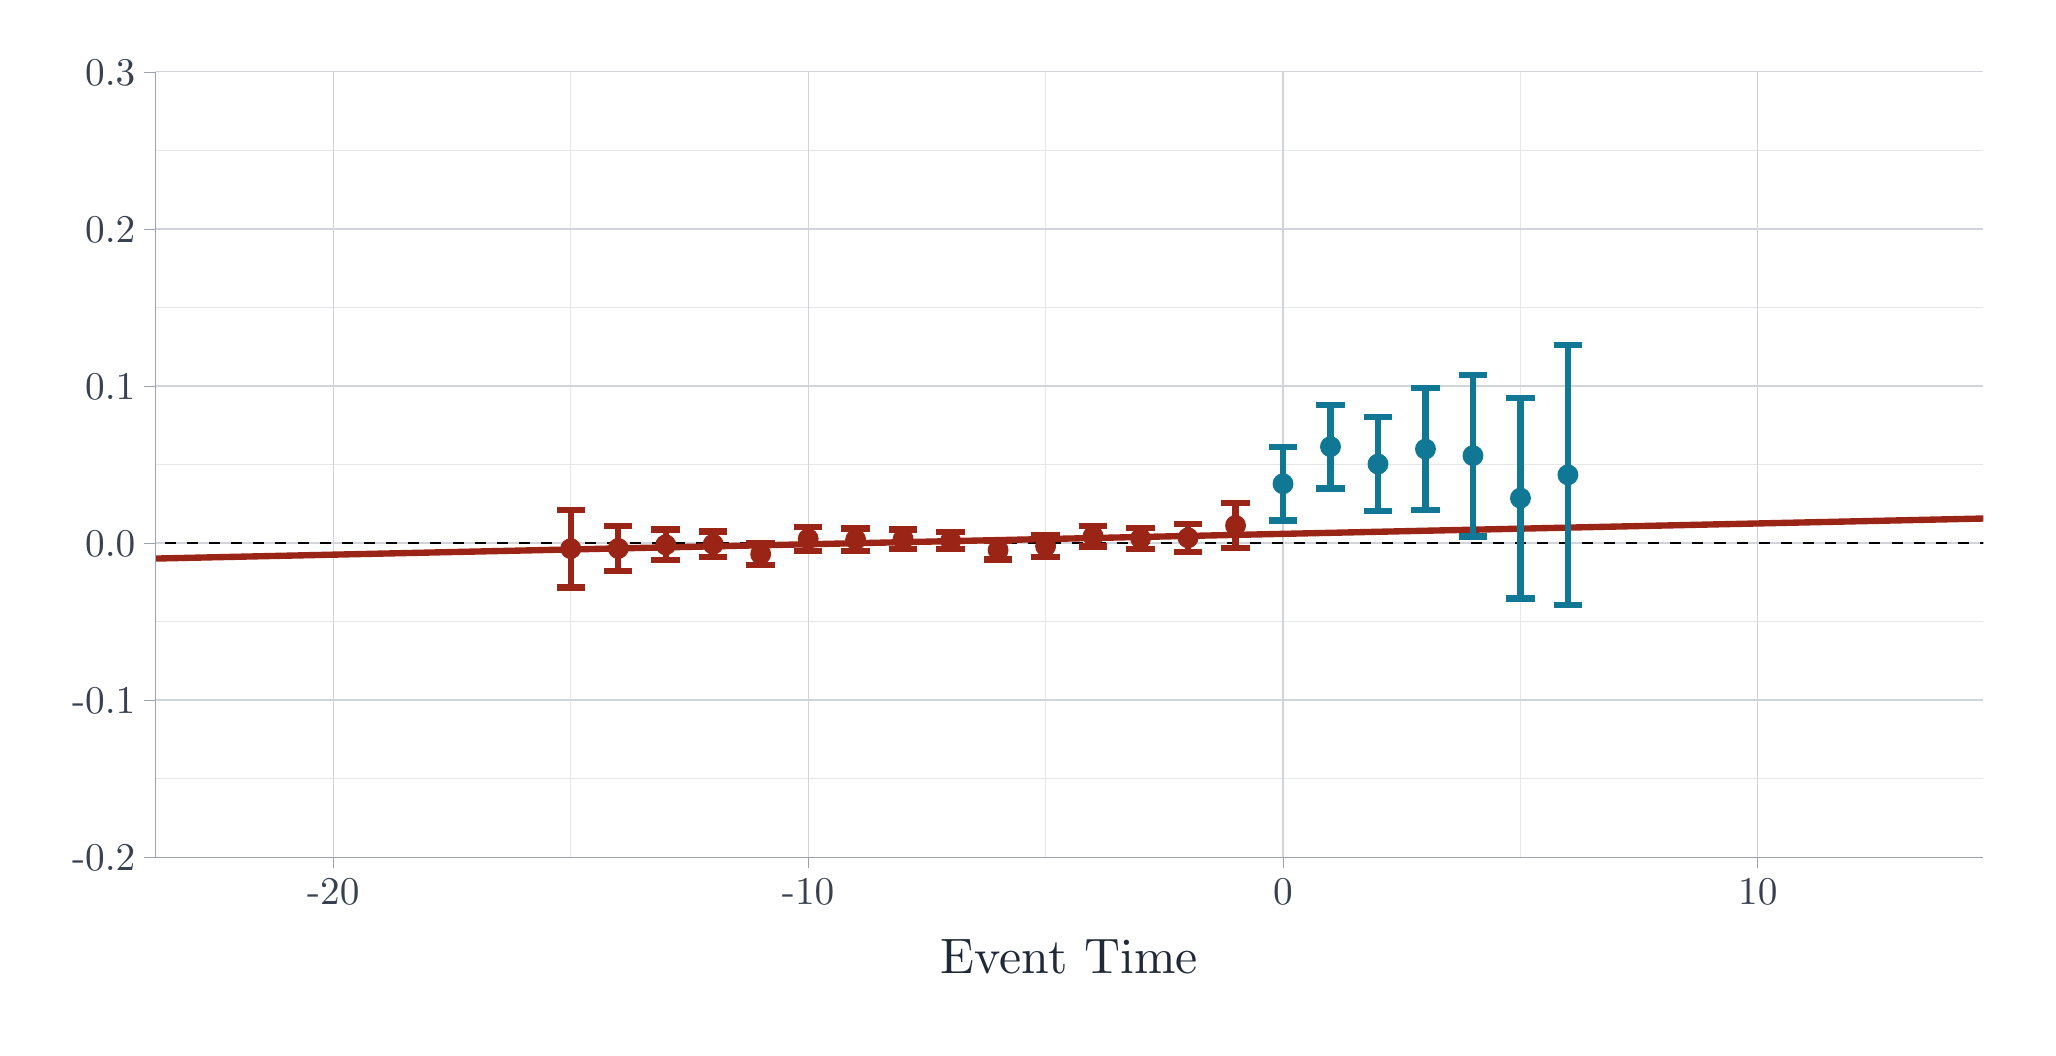
\begin{tikzpicture}[x=1pt,y=1pt]
\definecolor{fillColor}{RGB}{255,255,255}
\path[use as bounding box,fill=fillColor] (0,0) rectangle (722.70,361.35);
\begin{scope}
\path[clip] (  0.00,  0.00) rectangle (722.70,361.35);
\definecolor{drawColor}{RGB}{255,255,255}

\path[draw=drawColor,line width= 0.8pt,line join=round,line cap=round,fill=fillColor] (  0.00,  0.00) rectangle (722.70,361.35);
\end{scope}
\begin{scope}
\path[clip] ( 46.10, 61.65) rectangle (706.70,345.35);
\definecolor{drawColor}{RGB}{255,255,255}
\definecolor{fillColor}{RGB}{255,255,255}

\path[draw=drawColor,line width= 0.8pt,line join=round,line cap=round,fill=fillColor] ( 46.10, 61.65) rectangle (706.70,345.35);
\definecolor{drawColor}{RGB}{229,231,235}

\path[draw=drawColor,line width= 0.2pt,line join=round] ( 46.10, 90.02) --
	(706.70, 90.02);

\path[draw=drawColor,line width= 0.2pt,line join=round] ( 46.10,146.76) --
	(706.70,146.76);

\path[draw=drawColor,line width= 0.2pt,line join=round] ( 46.10,203.50) --
	(706.70,203.50);

\path[draw=drawColor,line width= 0.2pt,line join=round] ( 46.10,260.24) --
	(706.70,260.24);

\path[draw=drawColor,line width= 0.2pt,line join=round] ( 46.10,316.98) --
	(706.70,316.98);

\path[draw=drawColor,line width= 0.2pt,line join=round] (196.24, 61.65) --
	(196.24,345.35);

\path[draw=drawColor,line width= 0.2pt,line join=round] (367.82, 61.65) --
	(367.82,345.35);

\path[draw=drawColor,line width= 0.2pt,line join=round] (539.41, 61.65) --
	(539.41,345.35);
\definecolor{drawColor}{RGB}{209,213,219}

\path[draw=drawColor,line width= 0.4pt,line join=round] ( 46.10, 61.65) --
	(706.70, 61.65);

\path[draw=drawColor,line width= 0.4pt,line join=round] ( 46.10,118.39) --
	(706.70,118.39);

\path[draw=drawColor,line width= 0.4pt,line join=round] ( 46.10,175.13) --
	(706.70,175.13);

\path[draw=drawColor,line width= 0.4pt,line join=round] ( 46.10,231.87) --
	(706.70,231.87);

\path[draw=drawColor,line width= 0.4pt,line join=round] ( 46.10,288.61) --
	(706.70,288.61);

\path[draw=drawColor,line width= 0.4pt,line join=round] ( 46.10,345.35) --
	(706.70,345.35);

\path[draw=drawColor,line width= 0.4pt,line join=round] (110.45, 61.65) --
	(110.45,345.35);

\path[draw=drawColor,line width= 0.4pt,line join=round] (282.03, 61.65) --
	(282.03,345.35);

\path[draw=drawColor,line width= 0.4pt,line join=round] (453.61, 61.65) --
	(453.61,345.35);

\path[draw=drawColor,line width= 0.4pt,line join=round] (625.20, 61.65) --
	(625.20,345.35);
\definecolor{drawColor}{RGB}{0,0,0}

\path[draw=drawColor,line width= 0.9pt,dash pattern=on 4pt off 4pt ,line join=round] (-614.49,175.13) -- (1367.30,175.13);
\definecolor{drawColor}{RGB}{154,36,21}

\path[draw=drawColor,line width= 2.3pt,line join=round] (-614.49,155.04) -- (1367.30,198.45);
\definecolor{fillColor}{RGB}{154,36,21}

\path[draw=drawColor,line width= 0.4pt,line join=round,line cap=round,fill=fillColor] (196.24,173.09) circle (  3.57);

\path[draw=drawColor,line width= 0.4pt,line join=round,line cap=round,fill=fillColor] (213.40,173.16) circle (  3.57);

\path[draw=drawColor,line width= 0.4pt,line join=round,line cap=round,fill=fillColor] (230.56,174.47) circle (  3.57);

\path[draw=drawColor,line width= 0.4pt,line join=round,line cap=round,fill=fillColor] (247.71,174.68) circle (  3.57);

\path[draw=drawColor,line width= 0.4pt,line join=round,line cap=round,fill=fillColor] (264.87,171.12) circle (  3.57);

\path[draw=drawColor,line width= 0.4pt,line join=round,line cap=round,fill=fillColor] (282.03,176.64) circle (  3.57);

\path[draw=drawColor,line width= 0.4pt,line join=round,line cap=round,fill=fillColor] (299.19,176.35) circle (  3.57);

\path[draw=drawColor,line width= 0.4pt,line join=round,line cap=round,fill=fillColor] (316.35,176.55) circle (  3.57);

\path[draw=drawColor,line width= 0.4pt,line join=round,line cap=round,fill=fillColor] (333.51,175.96) circle (  3.57);

\path[draw=drawColor,line width= 0.4pt,line join=round,line cap=round,fill=fillColor] (350.66,172.57) circle (  3.57);

\path[draw=drawColor,line width= 0.4pt,line join=round,line cap=round,fill=fillColor] (367.82,173.99) circle (  3.57);

\path[draw=drawColor,line width= 0.4pt,line join=round,line cap=round,fill=fillColor] (384.98,177.60) circle (  3.57);

\path[draw=drawColor,line width= 0.4pt,line join=round,line cap=round,fill=fillColor] (402.14,176.81) circle (  3.57);

\path[draw=drawColor,line width= 0.4pt,line join=round,line cap=round,fill=fillColor] (419.30,177.01) circle (  3.57);

\path[draw=drawColor,line width= 0.4pt,line join=round,line cap=round,fill=fillColor] (436.46,181.47) circle (  3.57);
\definecolor{drawColor}{RGB}{16,120,149}
\definecolor{fillColor}{RGB}{16,120,149}

\path[draw=drawColor,line width= 0.4pt,line join=round,line cap=round,fill=fillColor] (453.61,196.53) circle (  3.57);

\path[draw=drawColor,line width= 0.4pt,line join=round,line cap=round,fill=fillColor] (470.77,209.94) circle (  3.57);

\path[draw=drawColor,line width= 0.4pt,line join=round,line cap=round,fill=fillColor] (487.93,203.67) circle (  3.57);

\path[draw=drawColor,line width= 0.4pt,line join=round,line cap=round,fill=fillColor] (505.09,209.09) circle (  3.57);

\path[draw=drawColor,line width= 0.4pt,line join=round,line cap=round,fill=fillColor] (522.25,206.70) circle (  3.57);

\path[draw=drawColor,line width= 0.4pt,line join=round,line cap=round,fill=fillColor] (539.41,191.36) circle (  3.57);

\path[draw=drawColor,line width= 0.4pt,line join=round,line cap=round,fill=fillColor] (556.56,199.76) circle (  3.57);
\definecolor{drawColor}{RGB}{154,36,21}

\path[draw=drawColor,line width= 2.3pt,line join=round] (191.09,187.08) --
	(201.39,187.08);

\path[draw=drawColor,line width= 2.3pt,line join=round] (196.24,187.08) --
	(196.24,159.09);

\path[draw=drawColor,line width= 2.3pt,line join=round] (191.09,159.09) --
	(201.39,159.09);

\path[draw=drawColor,line width= 2.3pt,line join=round] (208.25,181.21) --
	(218.55,181.21);

\path[draw=drawColor,line width= 2.3pt,line join=round] (213.40,181.21) --
	(213.40,165.12);

\path[draw=drawColor,line width= 2.3pt,line join=round] (208.25,165.12) --
	(218.55,165.12);

\path[draw=drawColor,line width= 2.3pt,line join=round] (225.41,179.99) --
	(235.70,179.99);

\path[draw=drawColor,line width= 2.3pt,line join=round] (230.56,179.99) --
	(230.56,168.95);

\path[draw=drawColor,line width= 2.3pt,line join=round] (225.41,168.95) --
	(235.70,168.95);

\path[draw=drawColor,line width= 2.3pt,line join=round] (242.57,179.24) --
	(252.86,179.24);

\path[draw=drawColor,line width= 2.3pt,line join=round] (247.71,179.24) --
	(247.71,170.12);

\path[draw=drawColor,line width= 2.3pt,line join=round] (242.57,170.12) --
	(252.86,170.12);

\path[draw=drawColor,line width= 2.3pt,line join=round] (259.73,175.14) --
	(270.02,175.14);

\path[draw=drawColor,line width= 2.3pt,line join=round] (264.87,175.14) --
	(264.87,167.09);

\path[draw=drawColor,line width= 2.3pt,line join=round] (259.73,167.09) --
	(270.02,167.09);

\path[draw=drawColor,line width= 2.3pt,line join=round] (276.88,180.94) --
	(287.18,180.94);

\path[draw=drawColor,line width= 2.3pt,line join=round] (282.03,180.94) --
	(282.03,172.34);

\path[draw=drawColor,line width= 2.3pt,line join=round] (276.88,172.34) --
	(287.18,172.34);

\path[draw=drawColor,line width= 2.3pt,line join=round] (294.04,180.42) --
	(304.34,180.42);

\path[draw=drawColor,line width= 2.3pt,line join=round] (299.19,180.42) --
	(299.19,172.28);

\path[draw=drawColor,line width= 2.3pt,line join=round] (294.04,172.28) --
	(304.34,172.28);

\path[draw=drawColor,line width= 2.3pt,line join=round] (311.20,180.02) --
	(321.50,180.02);

\path[draw=drawColor,line width= 2.3pt,line join=round] (316.35,180.02) --
	(316.35,173.07);

\path[draw=drawColor,line width= 2.3pt,line join=round] (311.20,173.07) --
	(321.50,173.07);

\path[draw=drawColor,line width= 2.3pt,line join=round] (328.36,179.06) --
	(338.65,179.06);

\path[draw=drawColor,line width= 2.3pt,line join=round] (333.51,179.06) --
	(333.51,172.86);

\path[draw=drawColor,line width= 2.3pt,line join=round] (328.36,172.86) --
	(338.65,172.86);

\path[draw=drawColor,line width= 2.3pt,line join=round] (345.52,176.01) --
	(355.81,176.01);

\path[draw=drawColor,line width= 2.3pt,line join=round] (350.66,176.01) --
	(350.66,169.13);

\path[draw=drawColor,line width= 2.3pt,line join=round] (345.52,169.13) --
	(355.81,169.13);

\path[draw=drawColor,line width= 2.3pt,line join=round] (362.68,177.83) --
	(372.97,177.83);

\path[draw=drawColor,line width= 2.3pt,line join=round] (367.82,177.83) --
	(367.82,170.15);

\path[draw=drawColor,line width= 2.3pt,line join=round] (362.68,170.15) --
	(372.97,170.15);

\path[draw=drawColor,line width= 2.3pt,line join=round] (379.83,181.33) --
	(390.13,181.33);

\path[draw=drawColor,line width= 2.3pt,line join=round] (384.98,181.33) --
	(384.98,173.86);

\path[draw=drawColor,line width= 2.3pt,line join=round] (379.83,173.86) --
	(390.13,173.86);

\path[draw=drawColor,line width= 2.3pt,line join=round] (396.99,180.56) --
	(407.29,180.56);

\path[draw=drawColor,line width= 2.3pt,line join=round] (402.14,180.56) --
	(402.14,173.05);

\path[draw=drawColor,line width= 2.3pt,line join=round] (396.99,173.05) --
	(407.29,173.05);

\path[draw=drawColor,line width= 2.3pt,line join=round] (414.15,182.03) --
	(424.45,182.03);

\path[draw=drawColor,line width= 2.3pt,line join=round] (419.30,182.03) --
	(419.30,171.99);

\path[draw=drawColor,line width= 2.3pt,line join=round] (414.15,171.99) --
	(424.45,171.99);

\path[draw=drawColor,line width= 2.3pt,line join=round] (431.31,189.54) --
	(441.60,189.54);

\path[draw=drawColor,line width= 2.3pt,line join=round] (436.46,189.54) --
	(436.46,173.40);

\path[draw=drawColor,line width= 2.3pt,line join=round] (431.31,173.40) --
	(441.60,173.40);
\definecolor{drawColor}{RGB}{16,120,149}

\path[draw=drawColor,line width= 2.3pt,line join=round] (448.47,209.77) --
	(458.76,209.77);

\path[draw=drawColor,line width= 2.3pt,line join=round] (453.61,209.77) --
	(453.61,183.30);

\path[draw=drawColor,line width= 2.3pt,line join=round] (448.47,183.30) --
	(458.76,183.30);

\path[draw=drawColor,line width= 2.3pt,line join=round] (465.63,225.03) --
	(475.92,225.03);

\path[draw=drawColor,line width= 2.3pt,line join=round] (470.77,225.03) --
	(470.77,194.85);

\path[draw=drawColor,line width= 2.3pt,line join=round] (465.63,194.85) --
	(475.92,194.85);

\path[draw=drawColor,line width= 2.3pt,line join=round] (482.78,220.73) --
	(493.08,220.73);

\path[draw=drawColor,line width= 2.3pt,line join=round] (487.93,220.73) --
	(487.93,186.62);

\path[draw=drawColor,line width= 2.3pt,line join=round] (482.78,186.62) --
	(493.08,186.62);

\path[draw=drawColor,line width= 2.3pt,line join=round] (499.94,231.20) --
	(510.24,231.20);

\path[draw=drawColor,line width= 2.3pt,line join=round] (505.09,231.20) --
	(505.09,186.99);

\path[draw=drawColor,line width= 2.3pt,line join=round] (499.94,186.99) --
	(510.24,186.99);

\path[draw=drawColor,line width= 2.3pt,line join=round] (517.10,235.86) --
	(527.40,235.86);

\path[draw=drawColor,line width= 2.3pt,line join=round] (522.25,235.86) --
	(522.25,177.53);

\path[draw=drawColor,line width= 2.3pt,line join=round] (517.10,177.53) --
	(527.40,177.53);

\path[draw=drawColor,line width= 2.3pt,line join=round] (534.26,227.62) --
	(544.55,227.62);

\path[draw=drawColor,line width= 2.3pt,line join=round] (539.41,227.62) --
	(539.41,155.10);

\path[draw=drawColor,line width= 2.3pt,line join=round] (534.26,155.10) --
	(544.55,155.10);

\path[draw=drawColor,line width= 2.3pt,line join=round] (551.42,246.76) --
	(561.71,246.76);

\path[draw=drawColor,line width= 2.3pt,line join=round] (556.56,246.76) --
	(556.56,152.75);

\path[draw=drawColor,line width= 2.3pt,line join=round] (551.42,152.75) --
	(561.71,152.75);

\path[] ( 46.10, 61.65) rectangle (706.70,345.35);
\end{scope}
\begin{scope}
\path[clip] (  0.00,  0.00) rectangle (722.70,361.35);
\definecolor{drawColor}{RGB}{156,163,175}

\path[draw=drawColor,line width= 0.3pt,line join=round] ( 46.10, 61.65) --
	( 46.10,345.35);
\end{scope}
\begin{scope}
\path[clip] (  0.00,  0.00) rectangle (722.70,361.35);
\definecolor{drawColor}{RGB}{55,65,81}

\node[text=drawColor,anchor=base east,inner sep=0pt, outer sep=0pt, scale=  1.42] at ( 38.90, 56.76) {-0.2};

\node[text=drawColor,anchor=base east,inner sep=0pt, outer sep=0pt, scale=  1.42] at ( 38.90,113.50) {-0.1};

\node[text=drawColor,anchor=base east,inner sep=0pt, outer sep=0pt, scale=  1.42] at ( 38.90,170.24) {0.0};

\node[text=drawColor,anchor=base east,inner sep=0pt, outer sep=0pt, scale=  1.42] at ( 38.90,226.97) {0.1};

\node[text=drawColor,anchor=base east,inner sep=0pt, outer sep=0pt, scale=  1.42] at ( 38.90,283.71) {0.2};

\node[text=drawColor,anchor=base east,inner sep=0pt, outer sep=0pt, scale=  1.42] at ( 38.90,340.45) {0.3};
\end{scope}
\begin{scope}
\path[clip] (  0.00,  0.00) rectangle (722.70,361.35);
\definecolor{drawColor}{RGB}{156,163,175}

\path[draw=drawColor,line width= 0.3pt,line join=round] ( 42.10, 61.65) --
	( 46.10, 61.65);

\path[draw=drawColor,line width= 0.3pt,line join=round] ( 42.10,118.39) --
	( 46.10,118.39);

\path[draw=drawColor,line width= 0.3pt,line join=round] ( 42.10,175.13) --
	( 46.10,175.13);

\path[draw=drawColor,line width= 0.3pt,line join=round] ( 42.10,231.87) --
	( 46.10,231.87);

\path[draw=drawColor,line width= 0.3pt,line join=round] ( 42.10,288.61) --
	( 46.10,288.61);

\path[draw=drawColor,line width= 0.3pt,line join=round] ( 42.10,345.35) --
	( 46.10,345.35);
\end{scope}
\begin{scope}
\path[clip] (  0.00,  0.00) rectangle (722.70,361.35);
\definecolor{drawColor}{RGB}{156,163,175}

\path[draw=drawColor,line width= 0.3pt,line join=round] ( 46.10, 61.65) --
	(706.70, 61.65);
\end{scope}
\begin{scope}
\path[clip] (  0.00,  0.00) rectangle (722.70,361.35);
\definecolor{drawColor}{RGB}{156,163,175}

\path[draw=drawColor,line width= 0.3pt,line join=round] (110.45, 57.65) --
	(110.45, 61.65);

\path[draw=drawColor,line width= 0.3pt,line join=round] (282.03, 57.65) --
	(282.03, 61.65);

\path[draw=drawColor,line width= 0.3pt,line join=round] (453.61, 57.65) --
	(453.61, 61.65);

\path[draw=drawColor,line width= 0.3pt,line join=round] (625.20, 57.65) --
	(625.20, 61.65);
\end{scope}
\begin{scope}
\path[clip] (  0.00,  0.00) rectangle (722.70,361.35);
\definecolor{drawColor}{RGB}{55,65,81}

\node[text=drawColor,anchor=base,inner sep=0pt, outer sep=0pt, scale=  1.42] at (110.45, 44.66) {-20};

\node[text=drawColor,anchor=base,inner sep=0pt, outer sep=0pt, scale=  1.42] at (282.03, 44.66) {-10};

\node[text=drawColor,anchor=base,inner sep=0pt, outer sep=0pt, scale=  1.42] at (453.61, 44.66) {0};

\node[text=drawColor,anchor=base,inner sep=0pt, outer sep=0pt, scale=  1.42] at (625.20, 44.66) {10};
\end{scope}
\begin{scope}
\path[clip] (  0.00,  0.00) rectangle (722.70,361.35);
\definecolor{drawColor}{RGB}{31,41,55}

\node[text=drawColor,anchor=base,inner sep=0pt, outer sep=0pt, scale=  1.80] at (376.40, 19.50) {Event Time};
\end{scope}
\end{tikzpicture}
